% Define global options
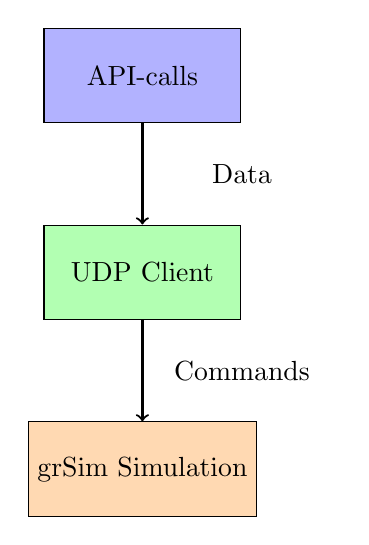
\begin{tikzpicture}[
    node distance=1.5cm and 2.5cm,
    every node/.style={align=center, minimum width=2.5cm, minimum height=1.2cm},
    api/.style={fill=blue!30},
    udp/.style={fill=green!30},
    grsim/.style={fill=orange!30}
]

    % Draw nodes
    \node[api, draw=black] (api) {API-calls};
    \node[udp, draw=black, below of=api, yshift=-1cm] (udp) {UDP Client};
    \node[grsim, draw=black, below of=udp, yshift=-1cm] (grsim) {grSim Simulation};
    
    % Draw connections
    \draw[->, thick] (api) -- (udp) node[midway, right] {Data};
    \draw[->, thick] (udp) -- (grsim) node[midway, right] {Commands};

\end{tikzpicture}